\documentclass[a4paper]{article}

%% Language and font encodings
\usepackage[english]{babel}
\usepackage[utf8x]{inputenc}
\usepackage[T1]{fontenc}
\usepackage[dvipsnames]{xcolor}
\definecolor{purple}{rgb}{0.5, 0.0, 0.5}
%% Sets page size and margins
\usepackage[a4paper,top=3cm,bottom=2cm,left=3cm,right=3cm,marginparwidth=1.75cm]{geometry}

%% Useful packages
\usepackage{amsmath}
\usepackage{graphicx}
\usepackage[colorinlistoftodos]{todonotes}
\usepackage[colorlinks=true, allcolors=blue]{hyperref}
\usepackage{float}
\usepackage{enumerate}
\usepackage{subfig}

\title{SQL}
\author{Ruonan Ji}

\begin{document}
\maketitle

\begin{abstract}
This is the notes that I take when study SQL, I am taking the course "The Complete SQL Bootcamp 2021: Go from Zero to Hero" from Udemy using pgAdmin 4.
\end{abstract}

\section{Before Start}

\begin{itemize}
  \item Create database: right click \textcolor{blue}{Databases}, \textcolor{blue}{Create}, \textcolor{blue}{Database...}, give a name to the new database, \textcolor{blue}{Save}.
  \item Delete database: close query tool window, right click the corresponding database, \textcolor{blue}{Delete/Drop}, \textcolor{blue}{Yes}.
  \item Shortcut to run code in query tool: F5 to run all the code, select partial code and F5 to run specific chunk of code.
  \item Find tables: click the using database, click \textcolor{blue}{Schemas}, under \textcolor{blue}{public} there is \textcolor{blue}{Tables}.
\end{itemize}

\section{Statement Fundamentals}
Cheat sheet for basic statements.\\
\newline
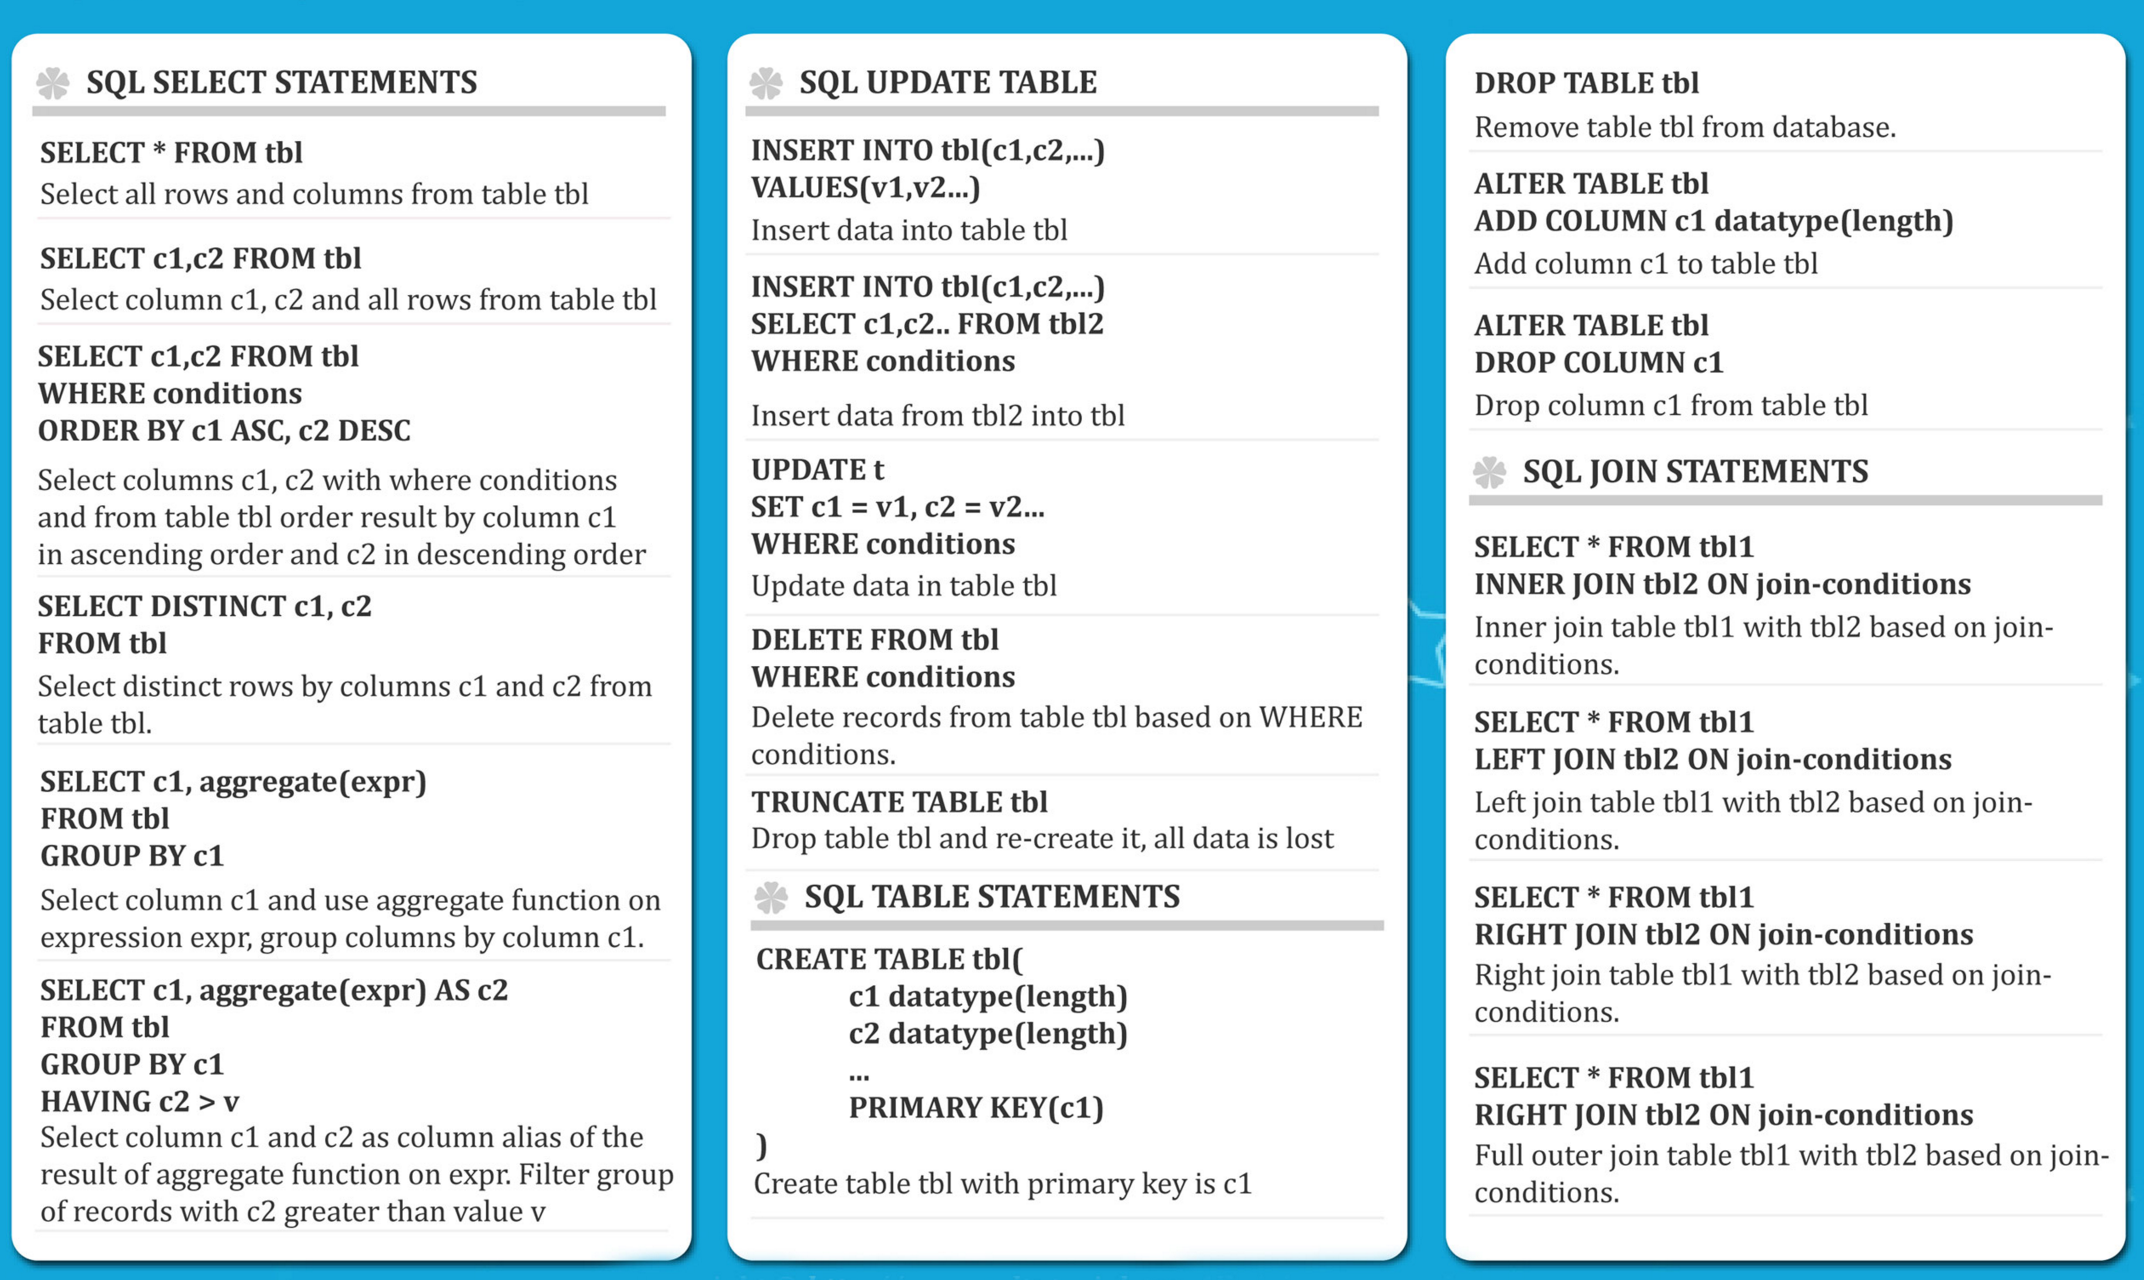
\includegraphics[scale=0.47]{cheat_sheet.png}
\subsection{SELECT Statement}
\begin{itemize}
  \item Usage: select certain columns from a table.
  \item Format: \textcolor{purple}{SELECT} c1, c2, c3 \textcolor{purple}{FROM} table;
\end{itemize}

\subsection{SELECT DISTINCT Statement}
\begin{itemize}
  \item Usage: only show distinct values in a certain column (no replication) from a table.
  \item Format: \textcolor{purple}{SELECT DISTINCT} c1 \textcolor{purple}{FROM} table;
  \item Extension: \textcolor{purple}{SELECT DISTINCT} c1, c2 \textcolor{purple}{FROM} table \textcolor{purple}{GROUP BY} c1, c2;
  \item Extension note: extract multiple cols with distinct value, the length of distinct values for each col should be the same, otherwise, there would be some values replicated.)
\end{itemize}

\subsection{COUNT Statement}
\begin{itemize}
  \item Usage: count the number of rows with the corresponding value from a table.
  \item Format: \textcolor{purple}{SELECT COUNT} (c1) \textcolor{purple}{FROM} table;
  \item Extension: \textcolor{purple}{SELECT COUNT} (c1) as new name \textcolor{purple}{FROM} table \textcolor{purple}{WHERE} c1 = the selected value
  \item Extension note: count the number of rows / frequency when c1 equal a specific value (the selected value) from the table. (recommend to always add () after COUNT, not sure why but sometimes gives me syntax error when I don't, but the problem will be fixed if I add ().)
\end{itemize}

\subsection{SELECT WHERE Statement}
\begin{itemize}
  \item Usage: select certain columns from a table.
  \item Format: \textcolor{purple}{SELECT} c1, c2, c3 \textcolor{purple}{FROM} table \textcolor{purple}{WHERE} condition;
  \item Under condition: comparison operators(>=,!=...), logical operators(AND/OR/NOT)
\end{itemize}

\subsection{ORDER BY Statement}
\begin{itemize}
  \item Usage: order the rows by columns in descending or ascending order.
  \item Format: \textcolor{purple}{SELECT} c1,c2,c3 \textcolor{purple}{FROM} table \textcolor{purple}{ORDER BY} c1 DESC;
  \item Extension: \textcolor{purple}{SELECT} c1,c2,c3 \textcolor{purple}{FROM} table \textcolor{purple}{ORDER BY} c1 DESC, c2 ASC;
  \item Extension note: order the rows first by c1 in descending order, then order by c2 in ascending order. (default order is ASC)
\end{itemize}

\subsection{LIMIT Statement}
\begin{itemize}
  \item Usage: only extract certain number of rows from a table.
  \item Format: \textcolor{purple}{SELECT} c1,c2 \textcolor{purple}{FROM} table \textcolor{purple}{WHERE} condition \textcolor{purple}{ORDER BY} c1 \textcolor{purple}{LIMIT} 5;
  \item Extension note: the order is very pivotal, I need to remember. I have tried to switch the order of the statements, but it shows syntax error. 
\end{itemize}

\subsection{BETWEEN AND Statement}
\begin{itemize}
  \item Usage: under \textcolor{purple}{WHERE} statement, use \textcolor{purple}{between} statement to set the range. It is same as <= value <= (inclusive). It can be used for date, time, number.
  \item Format: \textcolor{purple}{SELECT} c1 \textcolor{purple}{FROM} table \textcolor{purple}{WHERE} c1 \textcolor{purple}{BETWEEN} value1 \textcolor{purple}{AND} value2;
  \item Extension: \textcolor{purple}{SELECT} c1 \textcolor{purple}{FROM} table \textcolor{purple}{WHERE} c1 \textcolor{purple}{NOT BETWEEN} value1 \textcolor{purple}{AND} value2;
  \item Extension note: not between mean select the rows that have values smaller than value1 or greater than value2. Be careful about the date with time (2020-08-08 22:23:11 is not included when \textcolor{purple}{BETWEEN} `2020-08-01' \textcolor{purple}{AND} `2020-08-08' because the hour is over 00:00:00. So always double check the output date!) 
\end{itemize}

\subsection{IN Statement}
\begin{itemize}
  \item Usage: only extract rows that have values which match the selected values.
  \item Format: \textcolor{purple}{SELECT} * \textcolor{purple}{FROM} table \textcolor{purple}{WHERE} c1 \textcolor{purple}{IN} (value1,value2,value3);
  \item Extension: \textcolor{purple}{SELECT} * \textcolor{purple}{FROM} table \textcolor{purple}{WHERE} c1 \textcolor{purple}{NOT IN} (value1,value2,value3);
  \item Extension note: select the rows that have values which do not match the selected values.
\end{itemize}

\subsection{LIKE / ILIKE Statement}
\begin{itemize}
  \item Usage: use the wildcard($\%$, $\_$) to write some general patterns in a string to find the corresponding values.
  \item Wildcard: $\%$ matches any sequence of characters, $\_$ matches any single character
  \item Statement: LIKE: case-sensitive, ILIKE: case-insensitive.
  \item Format: \textcolor{purple}{SELECT} * \textcolor{purple}{FROM} table \textcolor{purple}{WHERE} c1 LIKE `her$\_$'; (herb)
  \item Format: \textcolor{purple}{SELECT} * \textcolor{purple}{FROM} table \textcolor{purple}{WHERE} c1 LIKE `$\_$her$\%$'; (Whether)  
  \item Format: \textcolor{purple}{SELECT} * \textcolor{purple}{FROM} table \textcolor{purple}{WHERE} c1 NOT LIKE `her$\_$'; (blablabla)
  \item Extension note: select the rows that have values which do not match the pattern.
\end{itemize}

\section{GROUP BY Statements}

\subsection{Aggregate Functions}
\begin{itemize}
  \item Usage: aggregate functions by using simple calculation.
  \item Common functions: AVG(), COUNT(), MAX(), MIN(), SUM().
  \item Format: \textcolor{purple}{SELECT} ROUND(\textcolor{purple}{AVG}(c1),2) \textcolor{purple}{FROM} table;
  \item Explanation: round up the average of values in c1 with 2 decimal places.
  \item Note: aggregate function calls happen only in the \textcolor{purple}{SELECT} clause or the \textcolor{purple}{HAVING} clause. If I want to select other cols in \textcolor{purple}{SELECT} clause, I should use \textcolor{purple}{GROUP BY}.
\end{itemize}

\subsection{GROUP BY Functions}
\begin{itemize}
  \item Usage: group rows that have same value, the column should be categorical.
  \item Format: \textcolor{purple}{SELECT} category col, \textcolor{purple}{AGG}(data col) \textcolor{purple}{FROM} table \textcolor{purple}{WHERE} category col != `A' \textcolor{purple}{GROUP BY} category col \textcolor{purple}{ORDER BY AGG}(data col);
  \item Note 1: the \textcolor{purple}{GROUP BY} clause must appear right after a \textcolor{purple}{FROM} or \textcolor{purple}{WHERE} statement.
  \item Note 2: columns in the \textcolor{purple}{SELECT} statement must be mentioned in \textcolor{purple}{GROUP BY} (aggregate functions are the exceptions, no need to be mentioned in group by).
  \item Note 3: \textcolor{purple}{WHERE} statement should not mention aggregate functions.
  \item Note 4: if I want to \textcolor{purple}{ORDER BY} aggregate functions, I have to reference the entire function like what I wrote in the format section.
  \item Note 5: the order of columns in \textcolor{purple}{GROUP BY} does not matter, but the order of columns in \textcolor{purple}{SELECT} matters.
\end{itemize}

\subsection{HAVING Functions}
\begin{itemize}
  \item Usage: filter aggregate functions.
  \item Format: \textcolor{purple}{SELECT} c1, \textcolor{purple}{SUM}(c2) \textcolor{purple}{FROM} table \textcolor{purple}{WHERE} c1 != `value' \textcolor{purple}{GROUP BY} c1 \textcolor{purple}{HAVING} \textcolor{purple}{SUM}(c2) > number;
  \item Note: I cannot use \textcolor{purple}{WHERE} to filter aggregate functions. Instead, I should use \textcolor{purple}{HAVING} right after \textcolor{purple}{GROUP BY} to condition aggregate functions.
\end{itemize}

\subsection{AS Functions}
\begin{itemize}
  \item Usage: output the variable name with a new name.
  \item Format: \textcolor{purple}{SELECT} c1, \textcolor{purple}{SUM}(c2) \textcolor{purple}{AS} total amount \textcolor{purple}{FROM} table \textcolor{purple}{WHERE} c1 != `value' \textcolor{purple}{GROUP BY} c1 \textcolor{purple}{HAVING} \textcolor{purple}{SUM}(c2) > number;
  \item Note: the new name only functions as an output name, it cannot be called as the original variable in any statement because it gets executed at the very end of a query. I have to call \textcolor{purple}{SUM}(c2) in \textcolor{purple}{HAVING} statement (Or c1 in \textcolor{purple}{WHERE} statement).
\end{itemize}

\section{JOINS}
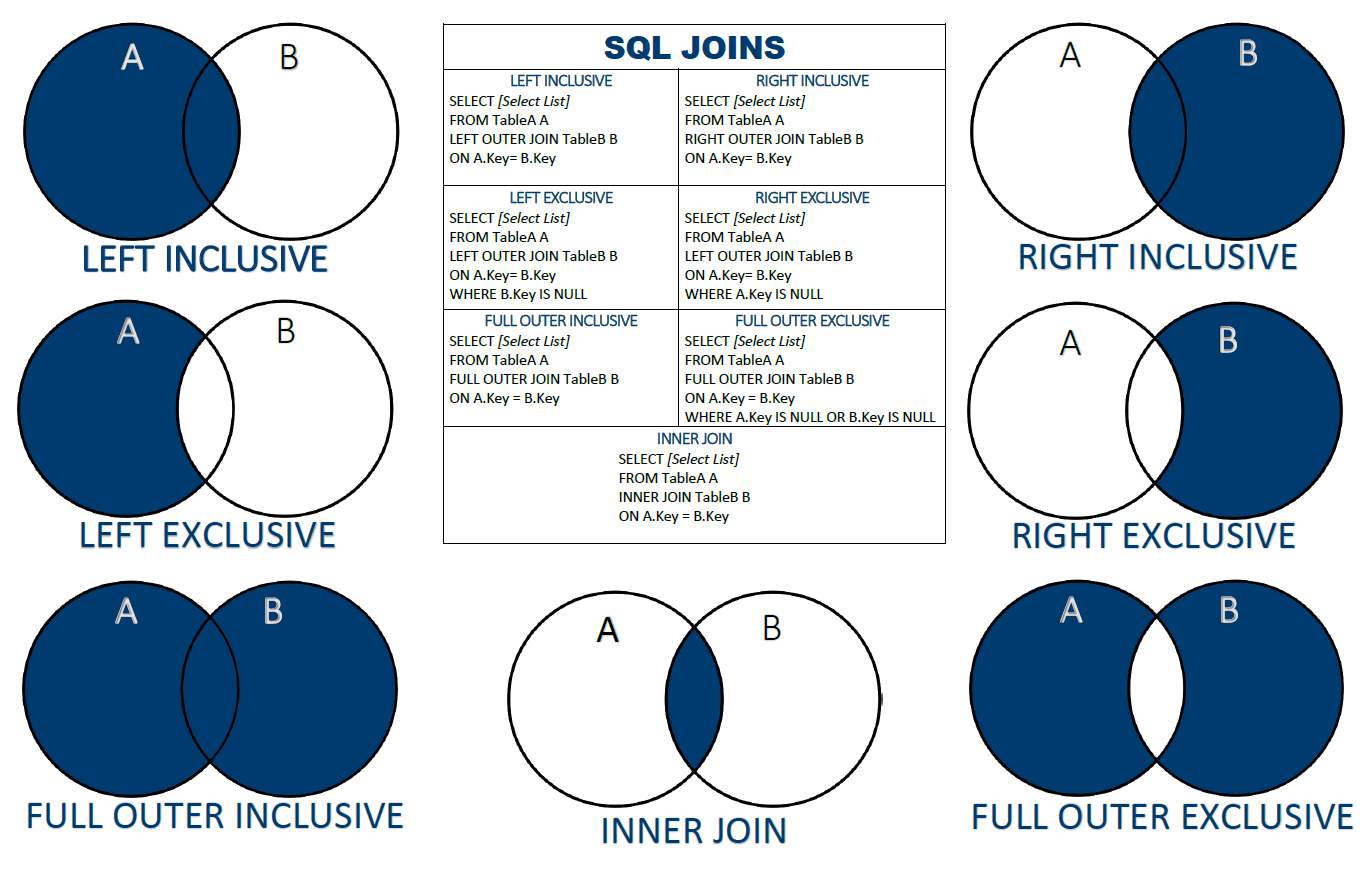
\includegraphics[scale=0.43]{joins.png}
\subsection{INNER JOINS}
\begin{itemize}
  \item Usage: get a new table that contains values which match in both tables.
  \item Format: \textcolor{purple}{SELECT} c1,tableA.c2,c3 \textcolor{purple}{FROM} tableA \textcolor{purple}{INNER JOIN} tableB \textcolor{purple}{ON} tableA.c2 = tableB.c2
  \item Note:  \textcolor{purple}{SELECT} c1,tableA.c2,c3 can eliminate duplicaion. Of course, I can just use \textcolor{purple}{SELECT} * if I do not care about duplication.
\end{itemize}

\subsection{FULL OUTER JOINS}
\begin{itemize}
  \item Usage: get a new table that contains all values from both tables.
  \item Format: \textcolor{purple}{SELECT} * \textcolor{purple}{FROM} tableA \textcolor{purple}{FULL OUTER JOIN} tableB \textcolor{purple}{ON} tableA.c2 = tableB.c2
  \item Note:  this is is for full outer inclusive graph. One important thing is if the values do not match, it will appear nulls!!!
  \item Extension: full outer exclusive graph excludes the common values from two tables, it always has nulls.
  \item Format: \textcolor{purple}{SELECT} * \textcolor{purple}{FROM} tableA \textcolor{purple}{FULL OUTER JOIN} tableB \textcolor{purple}{ON} tableA.c2 = tableB.c2 \textcolor{purple}{WHERE} tableA.c2 \textcolor{purple}{IS} null \textcolor{purple}{OR} tableB.c2 \textcolor{purple}{IS} null
\end{itemize}

\subsection{LEFT OUTER JOINS}
\begin{itemize}
  \item Usage: get a new table that contains all values from one table.
  \item Format: \textcolor{purple}{SELECT} * \textcolor{purple}{FROM} tableA \textcolor{purple}{LEFT OUTER JOIN} tableB \textcolor{purple}{ON} tableA.c2 = tableB.c2
  \item Note:  this is is for left inclusive graph. One important thing is if the values in tableB do not match values in tableA, the new table will appear nulls in tableB.
  \item Extension: left exclusive graph excludes the common values from two tables, it always has nulls.
  \item Format: \textcolor{purple}{SELECT} * \textcolor{purple}{FROM} tableA \textcolor{purple}{LEFT OUTER JOIN} tableB \textcolor{purple}{ON} tableA.c2 = tableB.c2 \textcolor{purple}{WHERE} tableB.c2 \textcolor{purple}{IS} null 
\end{itemize}

\subsection{RIGHT OUTER JOINS}
\begin{itemize}
  \item Usage: get a new table that contains all values from one table.
  \item Format: \textcolor{purple}{SELECT} * \textcolor{purple}{FROM} tableA \textcolor{purple}{RIGHT OUTER JOIN} tableB \textcolor{purple}{ON} tableA.c2 = tableB.c2
  \item Note:  this is is for right inclusive graph. One important thing is if the values in tableA do not match values in tableB, the new table will appear nulls in tableA.
  \item Extension: right exclusive graph excludes the common values from two tables, it always has nulls.
  \item Format: \textcolor{purple}{SELECT} * \textcolor{purple}{FROM} tableA \textcolor{purple}{RIGHT OUTER JOIN} tableB \textcolor{purple}{ON} tableA.c2 = tableB.c2 \textcolor{purple}{WHERE} tableA.c2 \textcolor{purple}{IS} null 
\end{itemize}

\subsection{UNION}
\begin{itemize}
  \item Usage: combine two or more \textcolor{purple}{SELECT} statements.
  \item Format: \textcolor{purple}{SELECT} c1 \textcolor{purple}{FROM} tableA \textcolor{purple}{UNION} \textcolor{purple}{SELECT} c1 \textcolor{purple}{FROM} tableB
  \item Note: the cols from tableA and tableB should match.
\end{itemize}

\section{Advanced SQL Commands}

\subsection{TIMESTAMPS and EXTRACT}
\begin{itemize}
  \item Usage: different forms of time.
  \item Format: \textcolor{purple}{SHOW} TIMEZONE / \textcolor{purple}{SELECT} NOW() / \textcolor{purple}{SELECT} TIMEOFDAY() / \textcolor{purple}{SELECT} CURRENT$\_$TIME / \textcolor{purple}{SELECT} CURRENT$\_$DAY
  \item Extension: date and time order: TIME, DATE, TIMESTAMP, TIMESTAMPTZ.
  \item Note: be careful when choosing level of TIMESTAMPTZ, I can always remove it  but cannot add it.
  \item functions 1: EXTRACT() extracts sub$\-$component from a col.
  \item Format 1: \textcolor{purple}{SELECT} \textcolor{purple}{EXTRACT} (YEAR/MONTH/DAY/WEEK/QUARTER \textcolor{purple}{FROM} c1) \textcolor{purple}{FROM} table
  \item functions 2: AGE() automatically calculates the current age given a timestamp.
  \item Format 2: \textcolor{purple}{SELECT} AGE (c1) \textcolor{purple}{FROM} table
  \item functions 3: TO$\_$CHAR converts data types to certain form of text.
  \item Format 3: \textcolor{purple}{SELECT} \textcolor{purple}{TO$\_$CHAR} (c1, `MONTH-YYYY') \textcolor{purple}{FROM} table
  \item link for data type formatting: https://www.postgresql.org/docs/12/functions-formatting.html
\end{itemize}

\subsection{Mathematical Functions and Operations}
\begin{itemize}
  \item Documentation for various signs: https://www.postgresql.org/docs/9.5/functions-math.html
  \item Format: \textcolor{purple}{SELECT} c1 $\%$ c2 \textcolor{purple}{AS} deposit \textcolor{purple}{FROM} table 
\end{itemize}

\subsection{String Functions and Operations}
\begin{itemize}
  \item Documentation for various signs: https://www.postgresql.org/docs/9.1/functions-string.html
  \item Format 1: \textcolor{purple}{SELECT} first$\_$name || ` ' || last$\_$name \textcolor{purple}{AS} fullname  \textcolor{purple}{FROM} table 
  \item Note 1: to concatenate first name and last name into one string with space between them.
  \item Format 2: \textcolor{purple}{SELECT} \textcolor{purple}{LOWER}(\textcolor{purple}{LEFT}(first$\_$name,1)) || \textcolor{purple}{LOWER}(last$\_$name) || `@gmail.com' \textcolor{purple}{AS} custom$\_$email  \textcolor{purple}{FROM} table 
  \item Note 2: to build a email address by picking the first letter of first name and concatenate with last name, lower the letters and adding @gmail.com at the end of the string.
\end{itemize}

\subsection{SubQuery}
\begin{itemize}
  \item Usage: performing a query on the results of another query (two \textcolor{purple}{SELECT} statements)
  \item Format 1: \textcolor{purple}{SELECT} c1 \textcolor{purple}{FROM} table.a \textcolor{purple}{WHERE} c1 \textcolor{purple}{IN} (\textcolor{purple}{SELECT} c1 \textcolor{purple}{FROM} table.b)
  \item Note 1: the subquery is inside the parenthesis and will be runed first. I can also use comparison operators and other commands instead of \textcolor{purple}{IN}.
  \item Extension 1: I can use \textcolor{purple}{JOINS} in the subquery.
  \item Format 2: \textcolor{purple}{SELECT} c1,c2 \textcolor{purple}{FROM} tablea \textcolor{purple}{AS} a \textcolor{purple}{WHERE} \textcolor{purple}{EXISTS} (\textcolor{purple}{SELECT} * \textcolor{purple}{FROM} tableb \textcolor{purple}{AS}  \textcolor{purple}{b} \textcolor{purple}{WHERE} \textcolor{purple}{b}.c3 = \textcolor{purple}{a}.c3) 
\end{itemize}

\section{Creating Databases and Tables}

\subsection{Data Types}
\begin{itemize}
  \item Documentation for data types: https://www.postgresql.org/docs/current/datatype.html
  \item Data types: Boolean (T/F), Character (char/varchar/text), Numeric (integer, floating-point number), Temporal(date, time, timestamp, interval), UUID, Array, JSON, Hstore key-value pair, special types such as network address and geometric data. 
  \item Note: Take time to plan for long term storage!
\end{itemize}

\subsection{Primary Keys}
\begin{itemize}
  \item Define: a primary key is a column or a group of columns used to identify a row uniquely in a table.
  \item Usage: primary keys are important since they allow us to easily discern what columns should be used for joining tables together.
  \item Note: when the table it shown, under a column name, if it says [PK], then the column is primary key. Moreover, the primary key contains values that are unique and non-null! (example: ID numbers, each person will have different ID to identify themselves from others.)
\end{itemize}

\subsection{Foreign Keys}
\begin{itemize}
  \item Define: a foreign key is a field or group of fields in a table that uniquely identifies a row in another table. 
  \item Note: the table that contains the foreign key is called referencing table or child table. The table to which the foreign key references is called referenced table or parent table. 
  \item Note: I can see which columns are primary keys and foreign keys by clicking "constraints" below "schemas"
\end{itemize}

\subsection{Constraints}
\begin{itemize}
  \item Define: constraints are the rules enforced on data columns on table. 
  \item Usage: it improves the accuracy and reliability of the data in the database by preventing invalid data from being entered into the database.
  \item Usage: column constraints: constrains the data in a columns to adhere to certain conditions; table constraints: applied to the entire table rather than to an individual column
  \item Note: common constraints: NOT NULL constraint, UNIQUE constraint, PRIMARY Key, FOREIGN Key, CHECK constraint, EXCLUSION constraint, REFERENCES, 
\end{itemize}

\subsection{CREATE Tables}
\begin{itemize}
  \item Format: \textcolor{purple}{CREATE TABLE} tbl$\_$name(user$\_$id \textcolor{blue}{SERIAL} \textcolor{purple}{PRIMARY KEY}, username \textcolor{blue}{VARCHAR}(50) \textcolor{purple}{UNIQUE NOT NULL}, created$\_$on \textcolor{blue}{TIMESTAMP} \textcolor{purple}{NOT NULL})
  \item Note: tbl$\_$name is the created table's name, user$\_$id, username and created$\_$on are the three columns, SERIAL, VARCHAR and TIMESTAMP are the data type from the column, PRIMARY KEY, UNIQUE and NOT NULL are the column constraints. 
  \item Extension: \textcolor{purple}{CREATE TABLE} account$\_$job(user$\_$id \textcolor{blue}{INTEGER} \textcolor{purple}{REFERENCES} account(user$\_$id), job$\_$id \textcolor{blue}{INTEGER} \textcolor{purple}{REFERENCES} job(job$\_$id), hire$\_$date \textcolor{blue}{TIMESTAMP})
  \item Note: account$\_$job is a reference table, user$\_$id and job$\_$id are foreign keys because they are originally from account table and job table. 
\end{itemize}

\subsection{INSERT}
\begin{itemize}
  \item Define: INSERT helps me add in rows to a table
  \item Note: the inserted row values must match up for the table, including constraints.
  \item Format: \textcolor{purple}{INSERT INTO} account(username, created$\_$on) \textcolor{purple}{VALUES} (`Jenna', \textcolor{purple}{CURRENT$\_$TIMESTAMP})
  \item Note: account is the table name. username and created$\_$on are column names from the table.
\end{itemize}

\subsection{UPDATE}
\begin{itemize}
  \item Define: UPDATE helps me change values of the columns in a table
  \item Format 1: \textcolor{purple}{UPDATE} account \textcolor{purple}{SET} c1 = \textcolor{purple}{CURRENT$\_$TIMESTAMP} \textcolor{purple}{WHERE} {c2 = 5}
  \item Note 1: account is the table name. c1 is the column name where values will be updated if meets the \textcolor{purple}{WHERE} condition.
  \item Format 2: \textcolor{purple}{UPDATE} account \textcolor{purple}{SET} original$\_$col = tableB.new$\_$col \textcolor{purple}{FROM} tableB \textcolor{purple}{WHERE} account.id = tableB.id
  \item Note 2: use another table's values by applying UPDATE join method.
  \item Format 3: \textcolor{purple}{UPDATE} account \textcolor{purple}{SET} last$\_$login = created$\_$on \textcolor{purple}{returning} account$\_$id, last$\_$login
  \item Note 3: only output affected rows
\end{itemize}

\subsection{DELETE}
\begin{itemize}
  \item Define: delete rows from a table
  \item Format: \textcolor{purple}{DELETE FROM} account \textcolor{purple}{WHERE} row$\_$id = 1
  \item Note: similar to UPDATE command, I can also add in a RETURNING call to output rows that have been deleted.
\end{itemize}

\subsection{ALTER}
\begin{itemize}
  \item Define: adding, dropping or renaming columns; changing a column's data type; set DEFAULT values for a column; add CHECK constraints; rename table
  \item Format: \textcolor{purple}{ALTER TABLE} account \textcolor{purple}{ADD COLUMN} new$\_$col \textcolor{purple}{TYPE}
  \item Note: the above format is just a simple example of adding a column. There are so many different ALTER commands. This website can give some basic ideas of what I can do with ALTER: https://www.java67.com/2013/01/how-to-use-alter-command-in-sql-examples.html.
\end{itemize}

\subsection{DROP}
\begin{itemize}
  \item Define: allows for the complete removal of a column in a table.
  \item Format 1: \textcolor{purple}{ALTER TABLE} account \textcolor{purple}{DROP COLUMN} c1
  \item Format 2: \textcolor{purple}{ALTER TABLE} account \textcolor{purple}{DROP COLUMN} c1 \textcolor{purple}{CASCADE} 
  \item Note 2: remove all dependencies: CASCADE clause is needed because DROP will not remove cols used in views, triggers or stored procedures.
  \item Format 3: \textcolor{purple}{ALTER TABLE} account \textcolor{purple}{DROP COLUMN IF EXISTS} c1
  \item Note 3: I consider this format as a useful, important tool. It is always safe to check for existence to avoid error.
  \item Format 4: \textcolor{purple}{ALTER TABLE} account \textcolor{purple}{DROP COLUMN} c1,  \textcolor{purple}{DROP COLUMN} c2, \textcolor{purple}{DROP COLUMN} c3
  \item Note 4: drop multiple cols.
\end{itemize}

\subsection{CHECK}
\begin{itemize}
  \item Define: the CHECK constraints are added when creating a table. The constraints allow me to create more customized constraints that adhere to a certain condition. 
  \item Format: \textcolor{purple}{CREATE TABLE} account (id \textcolor{blue}{SERIAL} \textcolor{purple}{PRIMARY KEY}, birthdate \textcolor{blue}{DATE} \textcolor{purple}{CHECK} (birthdate > `1900-01-01'), hiredate \textcolor{blue}{DATE} \textcolor{purple}{CHECK} (hiredate > birthdate))
  \item Note: when INSERT values into the created table, if the values violate the CHECK constraints, it will produce an error that warns me the values are not appropriate.
\end{itemize}

\section{Conditional Expressions and Procedures}
\subsection{Case}
\begin{itemize}
  \item Define: CASE statement works like if...else... statement. 
  \item Note: there are two main ways: a general CASE; a CASE expression.
  \item Format 1: \\
  \textcolor{purple}{SELECT} c1,
  \\\textcolor{purple}{CASE}\\\textcolor{purple}{WHEN} (c1 <= 100) \textcolor{purple}{THEN} `a'\\\textcolor{purple}{WHEN} (c1 \textcolor{purple}{BETWEEN 1 AND 10} \textcolor{purple}{THEN} `b')\\\textcolor{purple}{ELSE} `c'\\\textcolor{purple}{END}\\\textcolor{purple}{FROM} tbl
  \item Note 1: (I failed to find a way to indent. It should be(select...from(case...end)(when...when...else...))) The above format is an example of a general CASE which for WHEN function can check conditions.
  \item Format 2: \\
  \textcolor{purple}{SELECT} c1,
  \\\textcolor{purple}{CASE} c1\\\textcolor{purple}{WHEN} 100 \textcolor{purple}{THEN} `a'\\\textcolor{purple}{WHEN} 10 \textcolor{purple}{THEN} `b'\\\textcolor{purple}{ELSE} `c'\\\textcolor{purple}{END}\\\textcolor{purple}{FROM} tbl
  \item Note 2: The above format is an example of a CASE expression which for WHEN function can check values' equality.
\end{itemize}

\subsection{COALESCE}
\begin{itemize}
  \item Define: the COALESCE function accepts an unlimited number of arguments and returns the first argument that is not null. 
  \item Format: \textcolor{purple}{SELECT} c1, (c3-COALESCE(c2,0)) \textcolor{purple}{AS} new$\_$col \textcolor{purple}{FROM} tbl  
  \item Note: null values from c2 will be replaced with 0s. This function is very useful when substitute null values with another value.
\end{itemize}

\subsection{CAST}
\begin{itemize}
  \item Define: the CAST function allows to convert from one data type into another, but the converting should be reasonable. (`5' to 5)
  \item Format 1: \textcolor{purple}{SELECT} \textcolor{purple}{CAST} (`5'\textcolor{purple}{AS} \textcolor{purple}{INTEGER}) \\ Another way of doing it: \textcolor{purple}{SELECT} `5':: \textcolor{purple}{INTEGER}
  \item Note 1: two ways of converting a string into an integer.
  \item Format 2: \textcolor{purple}{SELECT} \textcolor{purple}{CAST} (c1\textcolor{purple}{AS} \textcolor{purple}{INTEGER}) \textcolor{purple}{FROM} tbl
  
\end{itemize}

\subsection{NULLIF}
\begin{itemize}
  \item Define: it takes in 2 arguments and return NULL if the arguments are equal to each other; return the first argument if the arguments are not equal. 
  \item Format: \textcolor{purple}{SELECT} c1/ \textcolor{purple}{NULLIF} (c2,0) \textcolor{purple}{FROM} tbl  
  \item Note: use NULLIF will prevent producing error when the denominator is 0. If c2 is 0, it will output `NULL', if c2 is not 0, it will output a normal division result.
\end{itemize}

\subsection{Views}
\begin{itemize}
  \item Define: a view acts more like defining a function in other coding languages. More specifically, stores a bunch of queries that I use frequently and create a temporary table that helps me extract certain data quickly. 
  \item Format:\\ \textcolor{purple}{CREATE VIEW} tbl \textcolor{purple}{AS}\\ \textcolor{purple}{SELECT} c1,c2,c3 \textcolor{purple}{FROM} tblAA\\
  \textcolor{purple}{INNER JOIN} tblBB\\
  \textcolor{purple}{ON} tblAA.c1 = tblBB.c1 
  \item Note: There are many ways to edit a view like changing its name, adding columns, deleting it. Explore them using google.  
\end{itemize}

\subsection{Import and Export}
\begin{itemize}
  \item Note: Explore them using google.  
\end{itemize}


\end{document}